\chapter{Phương pháp đề xuất}
\label{Chapter3}

\section{Phát biểu bài toán}
\label{sec:problem_statement}

Như đã đề cập tại Mục~\ref{sec:research_urgency} và được hệ thống hóa qua các phân tích ở Chương~\ref{Chapter2}, việc trả lời hai câu hỏi nghiên cứu đặt ra ở Chương~\ref{Chapter1} đòi hỏi phải giải quyết đồng thời hai bài toán. Thứ nhất, xây dựng một độ đo định lượng nhạy cảm với hiện tượng chuyển giao tiêu cực (negative transfer), và có khả năng phản ánh mức độ đóng góp (tích cực hay tiêu cực) của quá trình thích ứng của các tri thức tiền nghiệm ẩn trong tham số khởi tạo chung $\theta_0$ trên tập hỗ trợ $S_i$. Thứ hai, dựa trên giá trị độ lợi chuyển giao, cần phải có một cơ chế hậu diễn giải có khả năng tổng hợp thông tin qua nhiều trạng thái tham số của quá trình thích ứng, điều mà chưa phương pháp nào hiện thời có thể đáp ứng cả ba tiêu chí đã nêu trong mục \ref{subsec:relatedwork_synthesis}.

Trước khi xây dựng độ đo định lượng hay một cơ chế cụ thể, ta xét bài toán diễn giải trên một mô hình dựa trên \acrshort{maml} đã hoàn tất giai đoạn meta-training. Mô hình này sở hữu bộ tham số khởi tạo chung $\theta_0$ thu được từ quá trình tối ưu hai cấp (bi-level optimization) theo phương trình~\eqref{eq:outer_loop} và \eqref{eq:inner_loop}. Với một tác vụ đích $\mathcal{T}_i$ bất kỳ tại thời điểm meta-testing, bao gồm một tập hỗ trợ $S_i = \{(x_k^S, y_k^S)\}_{k=1}^{N\times K}$ và tập truy vấn $Q_i = \{(x_k^Q, y_k^Q)\}_{k=1}^{M}$, quá trình thích ứng nhanh sinh ra một quỹ đạo tham số gồm $T+1$ trạng thái liên tiếp sau theo đúng quy tắc cập nhật inner-loop~\eqref{eq:inner_loop}.

\begin{equation}
    \phi_{0} = \theta_0 \;\longrightarrow\; \phi_{1} \;\longrightarrow\; \cdots \;\longrightarrow\; \phi_{T} = \phi_i^*,
    \label{eq:trajectory}
\end{equation}

Với $F$ là không gian đặc trưng chung mà $\phi_i^*$ và $\theta_0$ cùng chia sẻ sau quá trình thích ứng nhanh, ta có thể phân rã mỗi trạng thái tham số $\phi_j$ trong quỹ đạo~\eqref{eq:trajectory} thành hai thành phần chức năng $\phi_j = (\phi_j^{b}, \phi_j^{h})$. Tương ứng với phần thân trích xuất đặc trưng (backbone) $\phi_j^{b}$ và phần đầu phân lớp (head) $\phi_j^{h}$, kế thừa từ phương pháp tiếp cận của Raghu và các cộng sự~\cite{raghu2019rapid} cũng như Oh và các cộng sự~\cite{oh2020boil}. Theo đó, hàm trích xuất đặc trưng $f_{\phi_j^{b}}: \mathcal{X} \rightarrow F$ ánh xạ một mẫu đầu vào $x$ về không gian đặc trưng chung $F$, trong khi hàm phân lớp $g_{\phi_j^{h}}: F \rightarrow \mathcal{Y}$ đưa ra quyết định cuối cùng dựa trên biểu diễn đã được trích xuất, sao cho $h_{\phi_j}(x) = g_{\phi_j^{h}} \circ f_{\phi_j^{b}}(x)$.

Đặc biệt, tại trạng thái khởi đầu $\phi_0 = \theta_0$, $F$ chính là không gian đặc trưng tiền nghiệm được hình thành từ giai đoạn meta-training. Trong khi đó, tại trạng thái cuối $\phi_T = \phi_i^*$, tuy cùng một không gian $F$ nhưng ít nhiều đã bị điều biến bởi $T$ bước cập nhật gradient chịu tác động trực tiếp từ tập hỗ trợ $S_i$. Nhờ việc $\phi_i^*$ và $\theta_0$ cùng chia sẻ trên một không gian $F$ duy nhất, mọi sự dịch chuyển giữa hai trạng thái này, dù là tái sử dụng đặc trưng (feature reuse) hay tái cấu trúc biểu diễn (representation change), đều có thể được quan sát và đối chiếu trực tiếp mà không cần một phép biến đổi trung gian nào khác.

Dựa trên sự phân rã này, bài toán diễn giải mà chúng tôi đặt ra không nhằm vào một trạng thái tham số đơn lẻ, như cách các phương pháp Grad-CAM cục bộ~\cite{selvaraju2020grad, uddin2025expert} chỉ trích xuất tại $\phi_T$, mà mục tiêu chính là \textbf{sự đóng góp thực sự của việc thích ứng phần thân trích xuất đặc trưng (backbone)} vào hiệu năng trên tác vụ đích.

Để cô lập đóng góp này, bên cạnh quỹ đạo thích ứng đầy đủ (full adaptation) $\{\phi_0, \phi_1, \dots, \phi_T\}$~\eqref{eq:trajectory}, ta xét thêm một quỹ đạo can thiệp (intervention) $\{\phi_0^{f}, \phi_1^{f}, \dots, \phi_T^{f}\}$, được sinh ra bằng cách chủ động đóng băng phần thân tại $\theta_0^{b}$ trong suốt $T$ bước, chỉ cho phép phần đầu phân lớp cập nhật theo quy tắc inner-loop~\eqref{eq:inner_loop}, tức $\phi_j^{f} = (\theta_0^{b}, \phi_j^{f,h})$ với mọi $j = 0, \dots, T$. Việc can thiệp này chính là sự hiện thực hóa giả thuyết \emph{tái sử dụng đặc trưng} (feature reuse) của Raghu và các cộng sự~\cite{raghu2019rapid}, đóng vai trò như một đường cơ sở (baseline) phản ánh phần hiệu năng mà mô hình đạt được \emph{mà không cần} backbone rời khỏi $\theta_0^{b}$. Trong khi đó, quỹ đạo đầy đủ $\{\phi_0, \dots, \phi_T\}$, nơi cả backbone lẫn head cùng thích ứng tự do, phản ánh khả năng \emph{tái cấu trúc biểu diễn} (representation change) như quan sát của Oh và các cộng sự~\cite{oh2020boil}.

Cụ thể hơn, với $h(\phi, Q_i)$ là hành vi dự đoán của mô hình trên tập truy vấn $Q_i$ khi được tham số hóa bởi $\phi$, hai câu hỏi nghiên cứu đặt ra ở Mục~\ref{sec:research_urgency} có thể được thu gọn về hai bài toán con có quan hệ nhân quả với nhau. Bài toán con thứ nhất đòi hỏi định lượng khoảng cách hiệu năng giữa $h(\phi_T^{f}, Q_i)$ (nhánh can thiệp, backbone đóng băng) và $h(\phi_T, Q_i) = h(\phi_i^*, Q_i)$ (nhánh thích ứng toàn bộ, không can thiệp) theo một cách nhạy cảm với $S_i$, thay vì chỉ dừng ở độ chính xác thô trên từng nhánh riêng lẻ. Nói cách khác, đại lượng cần đo không phải là hiệu năng tuyệt đối sau thích ứng, mà là \emph{phần chênh lệch do chính backbone rời khỏi $\theta_0^{b}$ mang lại}. Nếu $h(\phi_T, Q_i) \approx h(\phi_T^{f}, Q_i)$, việc thích ứng backbone gần như không tạo thêm giá trị so với khi bị can thiệp đóng băng. Nếu $h(\phi_T, Q_i)$ vượt trội hơn $h(\phi_T^{f}, Q_i)$, sự tái cấu trúc biểu diễn mang lại chuyển giao tích cực. Ngược lại, nếu $h(\phi_T, Q_i)$ kém hơn $h(\phi_T^{f}, Q_i)$, chính việc thích ứng backbone dưới áp lực của $S_i$ là nguyên nhân gây ra chuyển giao tiêu cực. Bài toán con thứ hai, dựa trên giả thiết rằng độ lợi đo được ở bài toán con thứ nhất là một đại lượng có thể quy kết (attributable), đòi hỏi truy vết ngược đại lượng đó về từng mẫu $(x_k^S, y_k^S) \in S_i$ và định vị chúng trên không gian đặc trưng $F$ tại từng trạng thái $\phi_j$ của quỹ đạo, thay vì chỉ xét tại điểm cuối $\phi_T$.

Việc phát biểu bài toán theo hướng này cho phép chúng tôi tránh được hạn chế cố hữu của các phương pháp diễn giải tĩnh (Mục~\ref{subsec:background_post_hoc}) vốn chỉ quan sát một lát cắt duy nhất của mô hình. Đồng thời, phương pháp đề xuất không đòi hỏi quyền truy cập vào dữ liệu meta-training như TL-XML~\cite{mitsuka2025tlxml}, do toàn bộ thông tin cần thiết, gồm cặp quỹ đạo $\{\phi_0, \dots, \phi_T\}$ và $\{\phi_0^{f}, \dots, \phi_T^{f}\}$, tập hỗ trợ $S_i$ và tập truy vấn $Q_i$, đều đã sẵn có ngay tại thời điểm meta-testing. Trên cơ sở phát biểu bài toán này, Mục~\ref{sec:adaptation_gain} tiếp theo sẽ trình bày chi tiết cách xây dựng độ lợi thích ứng $\Delta M$ nhằm giải quyết bài toán con thứ nhất, trước khi Mục~\ref{sec:fama} trình bày cơ chế \acrshort{fama} nhằm giải quyết bài toán con thứ hai.

\section{Độ lợi thích ứng}
\label{sec:adaptation_gain}

Như đã trình bày ở Mục~\ref{sec:problem_statement}, bài toán con thứ nhất đòi hỏi một đại lượng có khả năng định lượng phần chênh lệch hiệu năng sinh ra bởi chính việc backbone rời khỏi $\theta_0^{b}$, thay vì đo hiệu năng tuyệt đối trên từng nhánh riêng lẻ. Để đại lượng này phục vụ được cả hai mục tiêu nghiên cứu đã nêu, chúng tôi đặt ra ba tiêu chí thiết kế bắt buộc.

\textbf{Thứ nhất, tính khả vi (differentiability).} Vì bài toán con thứ hai đòi hỏi cần có cơ chế truy ngược sự đóng góp của đại lượng này về từng mẫu trong $S_i$ thông qua lan truyền ngược qua quỹ đạo thích ứng. Do đó độ đo này không thể là một đại lượng rời rạc như độ chính xác (accuracy), mà phải liên tục và khả vi theo tham số $\phi$.

\textbf{Thứ hai, tính nhạy cảm với chuyển giao tiêu cực (sensitivity to negative transfer).} Độ đo phải phản ánh được \emph{chiều hướng} của đóng góp, tức là nó cần phân biệt rõ ràng giữa trường hợp việc thích ứng backbone mang lại lợi ích (positive transfer), gây hại (negative transfer), hay không tạo thêm giá trị (feature reuse) so với việc chỉ tái sử dụng đặc trưng sẵn có. Điều này loại trừ các độ đo chỉ đo độ lớn tuyệt đối của sự thay đổi (như khoảng cách biểu diễn CCA/CKA) mà không cho biết thay đổi đó tốt hay xấu cho tác vụ đích.

\textbf{Thứ ba, tính tổng quát (generality).} Độ đo không được ràng buộc vào một kiến trúc, hay một tập dữ liệu cụ thể, mà phải được biểu diễn dưới dạng kỳ vọng trên toàn bộ tác vụ $\mathcal{T}_i$ tại thời điểm meta-testing, nhất quán với cách \acrshort{maml} được đánh giá (Phương trình~\eqref{eq:outer_loop}).

\subsection{Định nghĩa}
\label{sec:definition_AG}

Dựa trên cơ sở của ba tiêu chí được đặt ra, với 
\begin{equation}
    \mathcal{L}(Q_i, \phi) := \frac{1}{M}\sum_{k=1}^{M} \ell\big(h_\phi(x_k^Q), y_k^Q\big)
    \label{eq:loss}
\end{equation}

là hàm mất mát trung bình (chẵng hạn như cross-entropy) được tính từ hành vi dự đoán $h(\phi, Q_i)$ đã định nghĩa ở Mục~\ref{sec:problem_statement} đối chiếu với nhãn thật trên tập truy vấn, chúng tôi định nghĩa \textbf{độ lợi thích ứng} (Adaptation Gain) như sau.

\begin{equation}
    \centering
    \Delta M := \mathbb{E}_{Q_i \sim \mathcal{T}_i} \Big[ \mathcal{L}(Q_i, \phi_T^{f}) - \mathcal{L}(Q_i, \phi_T) \Big],
    \label{eq:adaptation_gain}
\end{equation}

trong đó $\phi_T = \phi_i^*$ là trạng thái cuối của quỹ đạo thích ứng đầy đủ, còn $\phi_T^{f} = (\theta_0^{b}, \phi_T^{f,h})$ là trạng thái cuối của quỹ đạo can thiệp với backbone bị đóng băng tại $\theta_0^{b}$, cả hai đều được sinh ra từ cùng một tập hỗ trợ $S_i$ theo quy tắc inner-loop~\eqref{eq:inner_loop}.

Định nghĩa~\eqref{eq:adaptation_gain} ngầm giả định rằng toàn bộ chênh lệch $\mathcal{L}(Q_i,\phi_T^f) - \mathcal{L}(Q_i,\phi_T)$ đến từ việc phần thân mạng (backbone) dịch chuyển khỏi $\theta_0^b$. Tuy nhiên, vì phần đầu phân lớp (head) ở hai nhánh cũng được cập nhật trên các quỹ đạo khác nhau ($\phi_j^h$ so với $\phi_j^{f,h}$). Dẫn tới, một vấn đề cần được làm rõ trước khi phân tích $\Delta M$: \emph{Liệu phần chênh lệch do bản thân phần đầu phân lớp (head) thích ứng khác nhau giữa hai nhánh có làm nhiễu tín hiệu backbone hay không?} 

Để giải quyết câu hỏi này, bằng khai triển Taylor bậc hai của $L(Q_i,\cdot)$ quanh $\theta_0$ (chi tiết tại Phụ lục~\ref{appendix:taylor_proof}), ta có thể phân rã $\Delta M$ thành

\begin{equation}
    \begin{split}
        \Delta M = & -\,\underbrace{\Big[g_b^\top \Delta b_T + \tfrac{1}{2}\Delta b_T^\top H_{bb} \Delta b_T + \Delta b_T^\top H_{bh} \Delta h_T\Big]}_{C_b \;-\; \text{đóng góp thuần của backbone}} \\
    &+ \underbrace{\Big[g_h^\top(\Delta h_T^f - \Delta h_T) + \tfrac{1}{2}\big({\Delta h_T^f}^\top H_{hh} \Delta h_T^f - \Delta h_T^\top H_{hh} \Delta h_T\big)\Big]}_{R_h \;-\; \text{dư sai lệch từ head}},
    \end{split}
    \label{eq:decomposition}
\end{equation}

với $g_b, g_h$ và $H_{bb}, H_{bh}, H_{hh}$ lần lượt là gradient và các khối Hessian của $L(Q_i,\cdot)$ tại $\theta_0$, còn $\Delta b_T, \Delta h_T, \Delta h_T^f$ là độ dịch chuyển tích lũy sau $T$ bước của mỗi nhánh.

Số hạng $R_h$ chỉ triệt tiêu tuyệt đối khi $\Delta h_T = \Delta h_T^f$, tức khi hai nhánh cho ra cùng một quỹ đạo head. Điều này chỉ chính xác tuyệ đối khi $T=1$, do hai nhánh khởi đầu từ cùng $\theta_0$ nên bước gradient head đầu tiên trùng nhau. Với $T>1$, hai nhánh dần tách khỏi nhau do backbone chỉ dịch chuyển ở nhánh đầy đủ, kéo theo $\Delta h_T \neq \Delta h_T^f$ và $R_h \neq 0$.

\begin{assumption}[Cơ chế thích ứng nhanh]
\label{asm:fast_adaptation}
Quá trình thích ứng nhanh của \acrshort{maml} vận hành với số bước $T$ nhỏ và tốc độ học $\alpha$ nhỏ, sao cho $T\alpha \ll 1$. Điều này đảm bảo trạng thái $\phi_T$ nằm đủ gần $\theta_0$ để khai triển Taylor bậc hai của $\mathcal{L}(Q_i,\cdot)$ quanh $\theta_0$ là một xấp xỉ cục bộ (local approximation) hợp lệ, tương tự như cách Grant và các cộng sự~\cite{grant2018recasting} đã chứng minh. Điều kiện này cũng chính là tiền đề cấu thành khái niệm thích ứng nhanh (fast-adaptation) cốt lõi của \acrshort{maml}~\cite{finn2017model}.
\end{assumption}

\begin{proposition}[Tính chủ đạo của đóng góp backbone]
\label{prop:decomposition}
Dưới Giả định ~\ref{asm:fast_adaptation}, ta có $C_b = O(T\alpha)$ trong khi $R_h = O\big((T\alpha)^2\big)$. Do đó,
\begin{equation}
    \Delta M = -C_b + O\big((T\alpha)^2\big),
    \label{eq:leading_order}
\end{equation}
Tức trong chế độ thích ứng nhanh, $\Delta M$ xấp xỉ tuyến tính đóng góp thuần của backbone. Phần dư do sự sai lệch quỹ đạo của phần đầu phân lớp (head) là một vô cùng bé bậc cao và không làm thay đổi chiều hướng (dấu) của $\Delta M$.
\end{proposition}

(\textit{Chứng minh chi tiết của Mệnh đề~\ref{prop:decomposition}, bao gồm khai triển Taylor đầy đủ, trường hợp $T=1$ (đẳng thức chính xác $R_h=0$), và lập luận quy nạp cho $T>1$ dẫn tới cận $R_h = O((T\alpha)^2)$, được trình bày chi tiết tại Phụ lục~\ref{appendix:taylor_proof}.}

Nhờ Mệnh đề~\ref{prop:decomposition}, dấu và độ lớn của $\Delta M$ có thể được diễn giải trực tiếp qua $C_b$ — đại lượng chỉ phụ thuộc vào độ dịch chuyển của backbone. Nếu $\Delta M > 0$ ($C_b < 0$), việc để backbone thích ứng tự do giúp giảm mất mát trên $Q_i$ — quá trình tái cấu trúc biểu diễn (representation change) mang lại \textbf{chuyển giao tích cực}. Ngược lại, nếu $\Delta M < 0$ ($C_b > 0$), tương đương với việc thích ứng backbone dưới áp lực của $S_i$ làm tăng mất mát trên $Q_i$ so với khi bị đóng băng — nguyên nhân trực tiếp của \textbf{chuyển giao tiêu cực}, dù $\theta_0^b$ vẫn đủ tốt nếu được giữ nguyên. Nếu $\Delta M \approx 0$ ($C_b \approx 0$), giả thuyết \textbf{tái sử dụng đặc trưng} (feature reuse) của Raghu và các cộng sự~\cite{raghu2019rapid} là đủ để giải thích hiệu năng đạt được.

Trong thực nghiệm, kỳ vọng $\mathbb{E}_{Q_i \sim \mathcal{T}_i}[\cdot]$ ở phương trình~\eqref{eq:adaptation_gain} được xấp xỉ Monte Carlo bằng trung bình $\Delta M$ trên một tập hợp lớn tác vụ lấy mẫu từ $\mathcal{T}_i$ tại thời điểm meta-testing, theo đúng cách thức đánh giá chuẩn của \acrshort{maml}.

\section{Phương pháp \acrfull{fama}}
\label{sec:fama}

\subsection{Ý tưởng tổng quan}
\label{subsec:fama_overview}
Độ lợi thích ứng $\Delta M$ (được xây dựng ở Mục~\ref{sec:adaptation_gain}) đã định lượng \emph{mức độ} lợi hay hại khi cho phép phần thân mạng (backbone) tự do thích ứng trên tập hỗ trợ. Tuy nhiên, bản thân $\Delta M$ chỉ là một đại lượng vô hướng (scalar) ở cấp độ tác vụ. Do đó, nó không thể hiện được \emph{thành phần nào} trong tập hỗ trợ $S_i$, hay cụ thể hơn là \emph{biễu diễn đặc trưng} nào trong không gian $F$, đã trực tiếp gây ra sự thay đổi đó. Việc định vị nguồn gốc của sự chuyển giao (tích cực hoặc tiêu cực) trên không gian ảnh chính là bài toán cốt lõi mà bài toán con thứ hai hướng tới giải quyết.

Về nguyên tắc, cách trực tiếp nhất để lan truyền $\Delta M$ (hay hiệu giữa $\mathcal{L}(Q_i,\phi_T)$ và $\mathcal{L}(Q_i,\phi_T^f)$) ngược về không gian điểm ảnh (pixel space) của $S_i$ là thực hiện tính đạo hàm $\partial \Delta M / \partial S_i$. Nhưng quá trình này đòi hỏi vi phân trực tiếp qua toàn bộ $T$ bước cập nhật của cả hai quỹ đạo (Backpropagation-Through-Time - BPTT). Việc này đã vấp phải hai rào cản chí mạng. \textbf{Thứ nhất}, về mặt tính toán, nó yêu cầu lưu trữ và vi phân qua đồ thị của $2T$ bước cập nhật, dẫn đến chi phí tăng tuyến tính theo thời gian $T$ nhưng lại toàn phương theo số lượng tham số $P$. \textbf{Thứ hai}, về mặt ngữ nghĩa, giá trị vi phân được truyền đến tận ảnh đầu vào thường mang nhược điểm cố hữu của của bản đồ nổi bật (vanilla saliency map) \cite{simonyan2014visualising} - nhiễu hạt, rời rạc theo từng điểm ảnh và đánh mất cấu trúc không gian. Đó cũng là lý do các phương pháp như Grad-CAM \cite{selvaraju2020grad} chọn cách trích xuất tín hiệu giải thích tại tầng đặc trưng tích chập cuối cùng thay vì tại điểm ảnh.

Để vượt qua các rào cản này, chúng tôi đề xuất phương pháp \textbf{\acrfull{fama}} như một cơ chế kết hợp nhằm kế thừa và mở rộng Grad-CAM. Phương pháp này thực hiện trích xuất tín hiệu (grab-cut) tại tầng đặc trưng, nhưng thay vì áp dụng trên một trạng thái tĩnh, \acrshort{fama} thực hiện phép trích xuất này một cách \emph{lặp đi lặp lại} tại trên từng tham số $\phi^{(t-1)}$ dọc theo quỹ đạo thích ứng. Sau đó, một kỹ thuật từ lý thuyết điều khiển tối ưu \cite{pontryagin1962mathematical} gọi là \textbf{phương pháp liên hợp} (adjoint method) được sử dụng để tổng hợp các tín hiệu cục bộ này với độ phức tạp tính toán chỉ xấp xỉ tuyến tính $\mathcal{O}(TP)$. Hình~\ref{fig:fama_pipeline} minh họa bức tranh tổng quan của toàn bộ quy trình.

\begin{figure}[h]
    \centering
    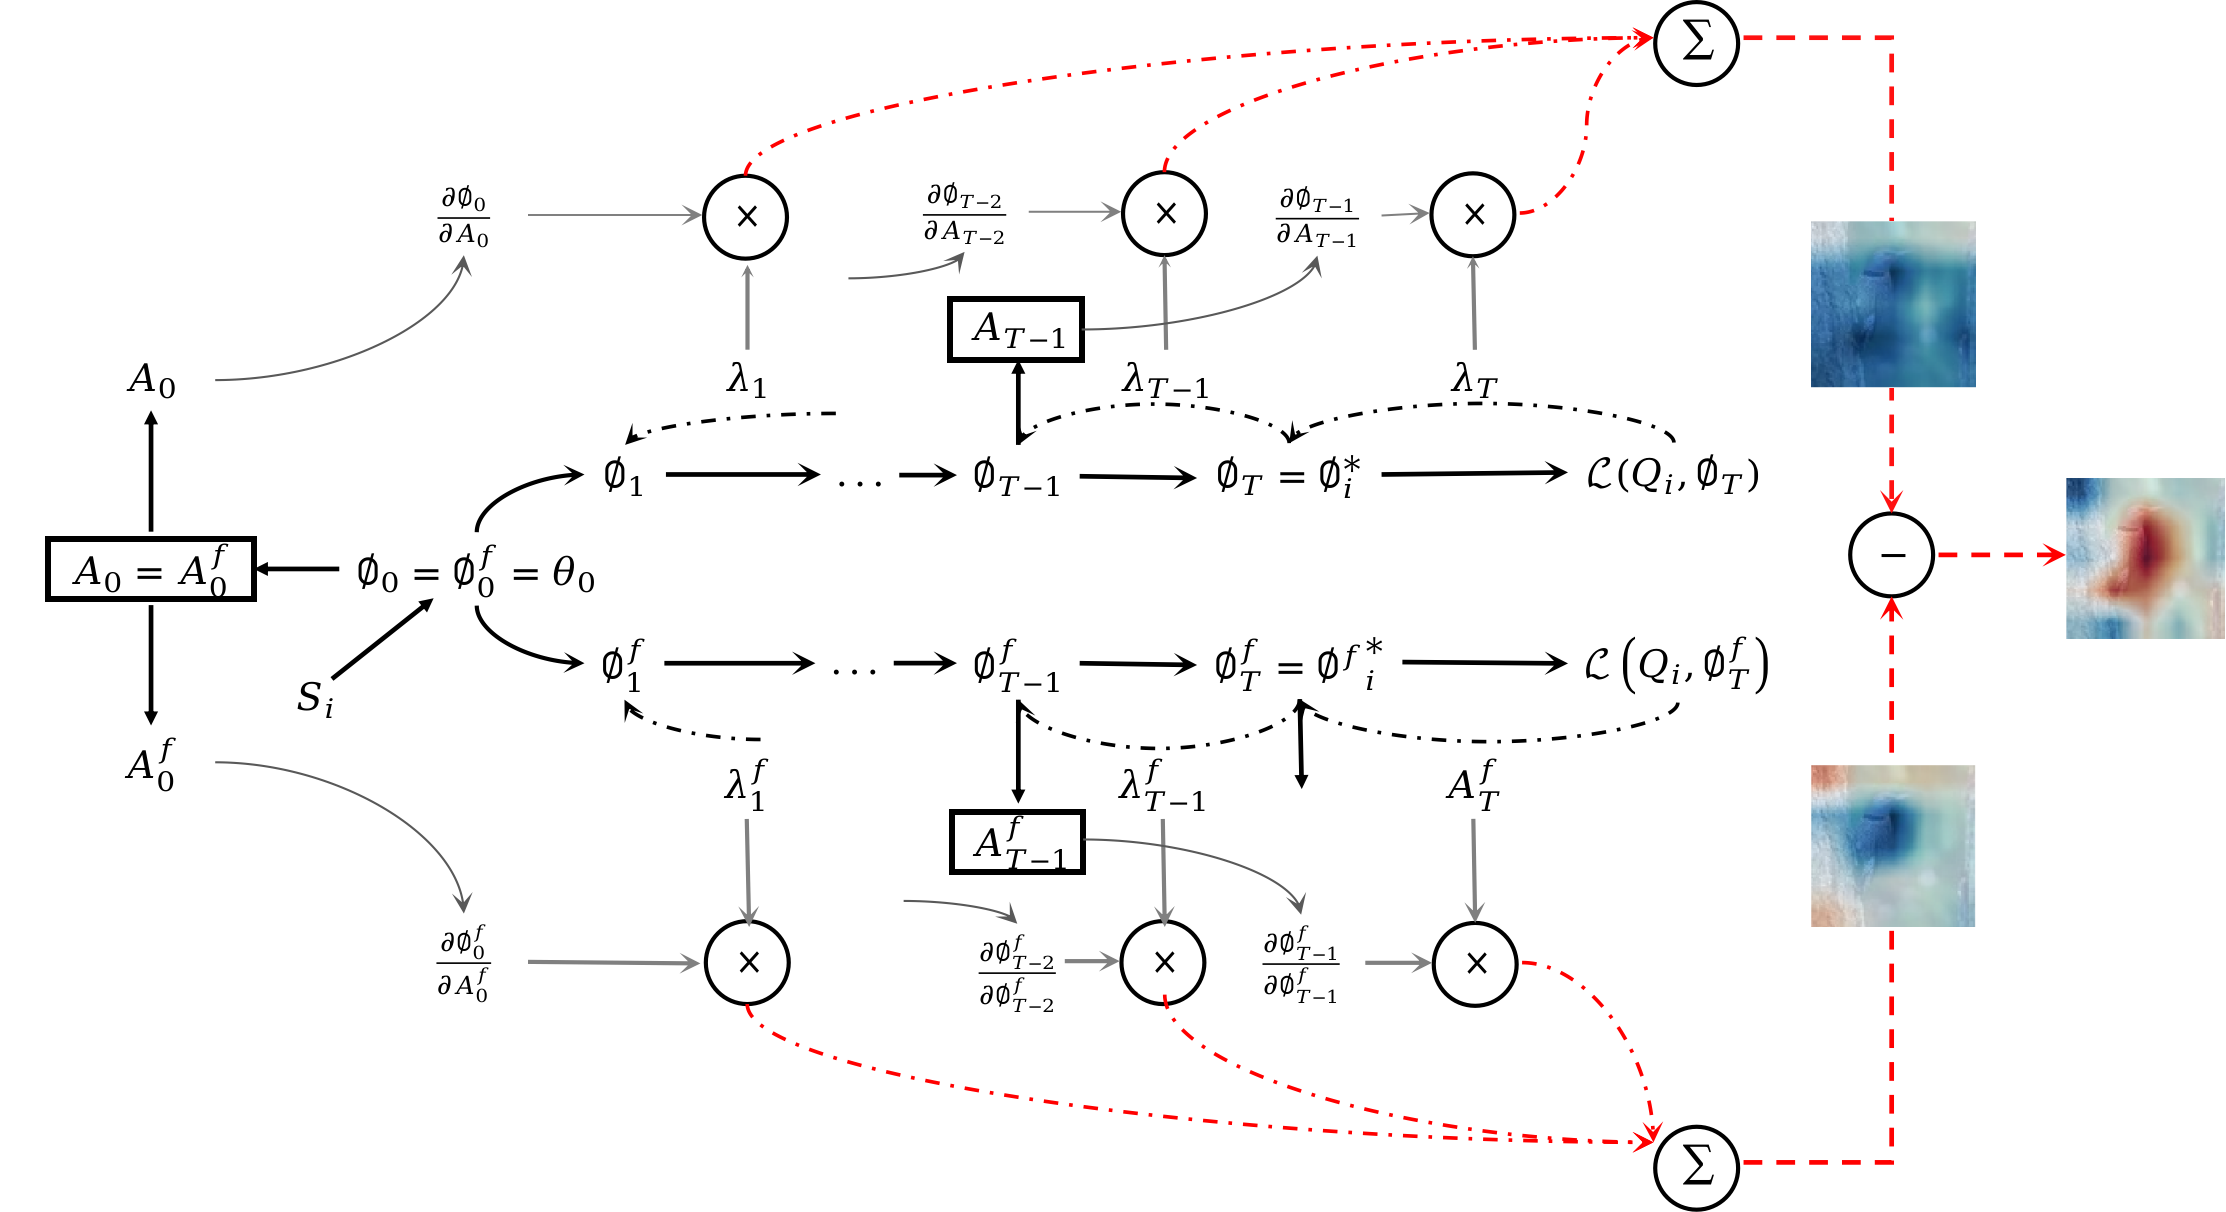
\includegraphics[width=0.9\textwidth]{../images/fama_pipeline.png}
    \caption{Pipeline tổng quan của \acrshort{fama}. Hai quỹ đạo (thích ứng toàn phần và can thiệp đóng băng) được sinh song song từ $S_i$; một lượt lan truyền ngược liên hợp duy nhất tính chuỗi $\{\lambda_t\}$ cho mỗi quỹ đạo; tại mỗi bước $t$, tín hiệu $\lambda_t$ được chiếu cục bộ lên bản đồ đặc trưng $A_{t-1}$; các bản đồ cục bộ được tích lũy theo $t$ rồi lấy hiệu giữa hai nhánh để ra bản đồ quy kết cuối cùng.}
    \label{fig:fama_pipeline}
\end{figure}

Để đảm bảo tính mạch lạc, phần còn lại của Mục~\ref{sec:fama} sẽ trình bày chi tiết theo trình tự bốn bước. (1) Khai triển đạo hàm quỹ đạo (Mục~\ref{subsec:derivative_expansion}). (2) Giải quyết chi phí tính toán bằng phương pháp liên hợp (Mục~\ref{subsec:adjoint}). (3) Định nghĩa đại lượng quy kết trên không gian đặc trưng (Mục~\ref{subsec:attribution_target}). và (4) Chiếu (projection) kết quả về không gian điểm ảnh (Mục~\ref{subsec:projection}).

\subsection{Khai triển đạo hàm qua quỹ đạo}
\label{subsec:derivative_expansion}
Xét một trong hai quỹ đạo (quá trình lập luận hoàn toàn tương tự đối với quỹ đạo còn lại). Gọi $g_{t-1} := \nabla_\phi \mathcal{L}(\phi_{(t-1)}, S_i)$ là gradient của hàm mất mát trên tập hỗ trợ. Theo quy tắc cập nhật vòng lặp trong (inner-loop) ở phương trình~\eqref{eq:inner_loop} cho $\phi_t = \phi_{t-1} - \alpha g_{t-1}$, ta thu được ma trận Jacobian cho một bước như sau.
\begin{equation}
    \frac{\partial \phi_t}{\partial \phi_{t-1}} = I - \alpha H_{t-1}, \qquad H_{t-1} := \nabla^2_\phi \mathcal{L}\big(\phi_{t-1}, S_i\big).
    \label{eq:step_jacobian}
\end{equation}

Theo đó, ta suy ra được vi phân trực tiếp qua thời gian (Backpropagation-Through-Time) bằng cách nhân dồn Jacobian từng bước qua toàn bộ $T$ bước cập nhật như sau.
\begin{equation}
    \frac{\partial \phi_T}{\partial \phi_0} = \prod_{t=1}^{T} \big(I - \alpha H_{t-1}\big),
    \label{eq:jacobian_product}
\end{equation}
Tích này tạo thành một ma trận có kích thước $P \times P$ (với $P$ là số lượng tham số trong mạng). Do đó, việc tính toán và lưu trữ tường minh ma trận này kéo theo chi phí bộ nhớ và thời gian lên đến $\mathcal{O}(TP^2)$, là một mức độ phức tạp hoàn toàn bất khả thi đối với các mạng nơ-ron học sâu.

Mặt khác, vì tập hỗ trợ $S_i$ đóng vai trò là đầu vào tường minh tại \emph{mọi} bước cập nhật. Nên theo quy tắc mắt xích (chain rule), đạo hàm của hàm mất mát đích $\mathcal{L}(Q_i, \phi_T)$ theo $S_i$ là tổng sự đóng góp của $S_i$ tại từng bước $t$.
\begin{equation}
    \frac{\partial \mathcal{L}(Q_i,\phi_{T})}{\partial S_i} \;=\; -\sum_{t=1}^{T} \alpha\, \lambda_t \cdot \frac{\partial^2 \mathcal{L}(\phi_{t-1}, S_i)}{\partial \phi_{t-1} \partial S_i},
    \label{eq:trajectory_expansion}
\end{equation}
trong đó $\lambda_t := \partial \mathcal{L}(Q_i,\phi_T)/\partial \phi_t$. (Được định nghĩa và chứng minh bằng quy nạp lùi tại Phụ lục~\ref{appendix:adjoint_proof}).

Mà từ cấu trúc phân rã ở phương trình~\eqref{eq:trajectory_expansion} này, có thể thấy được đạo hàm toàn cục của $\mathcal{L}(Q_i,\phi_T)$ hoàn toàn có thể chia tách thành $T$ số hạng cục bộ. Mà trong đó mỗi số hạng được đánh trọng số bởi $\lambda_t$. Dù vậy, bài toán tính $\lambda_t$ vẫn phải đối mặt với mức chi phí khổng lồ $\mathcal{O}(TP^2)$ nếu thực hiện khai triển Jacobian trực tiếp.

\subsection{Phương pháp liên hợp}
\label{subsec:adjoint}

Để vượt qua trở ngại về chi phí tính toán và bộ nhớ khi đánh giá ma trận Jacobian dọc theo quỹ đạo học, chúng tôi xây dựng cơ chế lan truyền dựa trên \emph{phương pháp trạng thái liên hợp} (Adjoint State Method). Nền tảng của phương pháp này xuất phát từ Nguyên lý cực đại Pontryagin trong lý thuyết điều khiển tối ưu.

Trong lý thuyết điều khiển liên tục, xét một hệ động lực với biến trạng thái $\mathbf{x}(t) = (x^1(t), \dots, x^n(t))$ và biến điều khiển $u(t)$ thay đổi theo hệ phương trình vi phân $\frac{dx^i}{dt} = f^i(\mathbf{x}(t), u(t))$. Để tính toán độ nhạy của một hàm mục tiêu tại thời điểm cuối $\Phi(\mathbf{x}(t_1))$ đối với sự thay đổi trạng thái ở một thời điểm $t$ bất kỳ, Pontryagin định nghĩa một vectơ liên hợp $\psi(t) = (\psi_1(t), \dots, \psi_n(t))$ tuân theo hệ phương trình liên hợp (adjoint system) ngược chiều thời gian:
\begin{equation}
    \frac{d\psi_i(t)}{dt} = - \sum_{\alpha=1}^n \frac{\partial f^\alpha(\mathbf{x}(t), u(t))}{\partial x^i} \psi_\alpha(t),
    \label{eq:pontryagin_continuous_component}
\end{equation}
hay được biểu diễn gọn dưới dạng ma trận Jacobian chuyển vị:
\begin{equation}
    \frac{d\psi(t)}{dt} = - \left( \frac{\partial f(\mathbf{x}(t), u(t))}{\partial \mathbf{x}} \right)^\top \psi(t),
    \label{eq:pontryagin_continuous}
\end{equation}
với điều kiện biên được khởi tạo tại điểm đích: $\psi(t_1) = \nabla_{\mathbf{x}} \Phi(\mathbf{x}(t_1))$. Hệ thức này cho phép lan truyền thông tin gradient từ tương lai về quá khứ mà không cần tính toán trực tiếp sự thay đổi tiến của toàn bộ quỹ đạo.

Trong ngữ cảnh của chúng tôi, quỹ đạo thời gian liên tục được rời rạc hóa thành các bước cập nhật tham số (gradient descent) $\phi_{t} = \phi_{t-1} - \alpha \nabla_{\phi} \mathcal{L}(\phi_{t-1})$. Lúc này, ma trận Jacobian của quá trình dịch chuyển đóng vai trò tương đương với toán tử tiến hóa $f$ của hệ thống, và vectơ liên hợp $\psi(t)$ của Pontryagin được chúng tôi ký hiệu và đối chiếu thành chuỗi biến rời rạc $\lambda_t$.

Quá trình tính toán chuỗi liên hợp $\{\lambda_t\}_{t=1}^T$ bắt đầu bằng việc khởi tạo điều kiện biên tại điểm cuối của quỹ đạo (tương đương $\psi(t_1)$):
\begin{equation}
    \lambda_T := \mathbb{E}_{Q_i \sim \mathcal{T}_i}\big[\nabla_\phi \mathcal{L}(Q_i, \phi_T)\big].
    \label{eq:adjoint_init}
\end{equation}
Đại lượng này được xấp xỉ bằng phương pháp Monte Carlo thông qua bootstrap phân tầng trên tập truy vấn $Q_i$. Từ mốc này, biến liên hợp $\lambda_t$ được lan truyền \emph{ngược} qua từng bước theo bản rời rạc hóa của phương trình~\eqref{eq:pontryagin_continuous}:
\begin{equation}
    \lambda_{t-1} = \lambda_t - \alpha\, H_{t-1}\, \lambda_t, \qquad t = T, T-1, \dots, 1.
    \label{eq:adjoint_recursion}
\end{equation}
trong đó $H_{t-1}$ là ma trận Hessian của hàm mất mát tại $\phi_{t-1}$.

\begin{proposition}[Tính tương đương của phép liên hợp]
\label{prop:adjoint_equivalence}
Với chuỗi $\lambda^{(t)}$ sinh ra bởi hệ phương trình~\eqref{eq:adjoint_init}--\eqref{eq:adjoint_recursion}, ta có đẳng thức thể hiện sự bảo toàn gradient: $\lambda^{(t)} = \partial \mathbb{E}_{Q_i}[\mathcal{L}(Q_i,\phi^{(T)})]/\partial \phi^{(t)}$ tại mọi bước $t = 0, 1, \dots, T$.
\end{proposition}

Từ mệnh đề~\ref{prop:adjoint_equivalence} ta hoàn toàn có thể thực hiện phép toán liên hợp nhằm tìm ra $\lambda_t$ tại mọi bước trong quỹ đạo mà không cần phải qua một chuỗi nhân Jacobian khổng lồ. Tuy nhiên, tính hợp lệ của phép tuyến tính hoá để đạt được hệ thức~\eqref{eq:adjoint_recursion} qua nhiều bước liên tiếp đòi hỏi các ràng buộc chặt chẽ về mặt không gian trạng thái sau.
 
\begin{assumption}[Tính trơn và ổn định của phép liên hợp]
\label{asm:adjoint_stability}
\leavevmode\newline\vspace{0.25em}
\begin{enumerate}[label=(\roman*)]
    \item $\mathcal{L}(\cdot, S_i)$ khả vi liên tục hai lần theo $\phi$ trong một lân cận mở chứa toàn bộ quỹ đạo $\{\phi_0, \dots, \phi_T\}$;
    \item Ma trận Hessian $H(\phi)$ thỏa mãn điều kiện liên tục Lipschitz, tức là tồn tại hằng số $L_H < \infty$ sao cho $\|H(\phi) - H(\phi')\| \le L_H \|\phi - \phi'\|$, đảm bảo sai số tuyến tính hoá tại mỗi bước bị chặn bởi $\mathcal{O}(\alpha^2)$;
    \item Tốc độ học $\alpha$ phải thỏa mãn bất đẳng thức $\alpha \le 2/\lambda_{\max}(H_{t-1})$ tại mọi bước $t$, nhằm đảm bảo toán tử $(I - \alpha H_{t-1})$ không giãn nở ($\|I - \alpha H_{t-1}\| \le 1$), từ đó ngăn hiện tượng chuỗi $\{\lambda_t\}$ bùng nổ qua $T$ bước lùi.
\end{enumerate}
\end{assumption}
Và với cơ chế thích ứng nhanh ($T\alpha \ll 1$), ta gần như hoàn toàn có thể thỏa mãn các ràng buộc này đối với các cấu trúc phổ trị riêng thông thường (chứng minh chi tiết tại Phụ lục~\ref{appendix:adjoint_proof}). 

Đồng thời khi chuyển sang hệ thức liên hợp~\eqref{eq:adjoint_recursion}, ta đã loại bỏ đi được rào cản về bộ nhớ bằng cách không cần phải lưu trữ và biểu diễn tường minh ma trận Hessian $H_{t-1}$ (vốn có kích thước rất lớn $P \times P$). Thay vào đó, quá trình này chỉ yêu tính trực tiếp \textbf{tích vô hướng Hessian-vector (HVP)}, $H_{t-1}\lambda_t$.

Để thực thi điều này, chúng tôi áp dụng kỹ thuật lan truyền ngược kép mà Pearlmutter đã đề xuất \cite{pearlmutter1994fast}. Đó là, thay vì tính ma trận Hessian $H$, ta hoàn toàn có thể tính đạo hàm có hướng (directional derivative) của gradient theo hướng của vector $\lambda_t$ như sau.
\begin{equation}
    H_{t-1}\lambda_t = \nabla_{\phi_{t-1}} \big\langle \nabla_{\phi_{t-1}} \mathcal{L}, \lambda_t \big\rangle
    \label{eq:hvp_trick}
\end{equation}
Tương đương với việc thực hiện hai lần lan truyền ngược (forward-over-reverse hoặc reverse-over-reverse) trong các triển khai thực tế. Với lần lan truyền đầu tiên tạo ra đồ thị tính toán cho tích vô hướng $\langle \nabla \mathcal{L}, \lambda_t \rangle$, và lần tiếp theo chính là lấy gradient của chính tích vô hướng đó.

Thông qua kỹ thuật HVP này, việc cập nhật $\lambda_{t-1}$ có thể được tính toán với chi phí không gian và thời gian tỷ lệ thuận với $\mathcal{O}(P)$. Kết quả là tổng chi phí qua $T$ bước được làm phẳng, giảm mạnh từ $\mathcal{O}(TP^2)$ xuống mức tuyến tính $\mathcal{O}(TP)$. Và chuỗi trọng số $\{\lambda^{(t)}\}$ thu được với chi phí thấp này sau đó sẽ đóng vai trò dẫn hướng cho việc quy kết trên không gian đặc trưng.

\subsection{Đại lượng quy kết}
\label{subsec:attribution_target}

Gọi $A_j := f_{\phi_j^{b}}(S_i) \in F$ trong đó $a_{jk}$ là biểu diễn đặc trưng của mẫu $x_k^S$ tại bước thứ $j$ của quỹ đạo (với kích thước $C \times H \times W$). Khác với các phương pháp giải thích tĩnh chỉ quan tâm đến một biểu diễn duy nhất ở cuối quỹ đạo $A_{T}$, \acrshort{fama} xử lý một \textbf{chuỗi biểu diễn} $\{A_0, \dots, A_{T-1}\}$, mỗi phần tử gắn với một trạng thái backbone khác nhau $\phi_j^{b}$ dọc theo quỹ đạo.

Do $A_j$ được tính toán lại từ đầu vào $S_i$ tại mỗi mốc thời gian thông qua một backbone $\phi_j^b$ không ngừng biến đổi, do đó không tồn tại một đại lượng $A$ toàn cục đóng vai trò trung gian cho toàn bộ quỹ đạo $T$ bước. Nói cách khác, thay vì có một phép biến đổi $S \to A \to \Delta M$ để có thể áp dụng quy tắc mắt xích một lần duy nhất, ta có $T$ phép biến đổi cục bộ tách biệt độc lập như sau. 
\begin{equation}
    S_i \xrightarrow{\ f_{\phi_{t-1}^{b}}\ } A_{t-1} \xrightarrow{\ } \mathcal{L}(\phi_{t-1}, S_i), \qquad t = 1, \dots, T,
    \label{eq:local_factorization}
\end{equation}

Nhận diện được cấu trúc này, \acrshort{fama} thực hiện cơ chế can thiệp cục bộ. Tại mỗi bước, bản đồ $A_{t-1}$ được ngắt khỏi mắt xích đạo hàm (stop-gradient), biến nó thành một biến lá (leaf variable) độc lập với toàn bộ lịch sử tính toán trước đó. Khi đó, đại lượng cần quy kết không còn là đạo hàm toàn cục, mà là một \textbf{họ} gồm $T$ giá trị phân bổ cục bộ.
\begin{equation}
    \mathrm{Attr}_{(t-1)} \;:=\; \frac{\partial}{\partial A_{(t-1)}}\Big[\lambda_t \cdot \nabla_{\phi} \mathcal{L}\big(\phi_{t-1}, S_i\big)\Big], \qquad t = 1,\dots,T,
    \label{eq:local_attr}
\end{equation}
Tại đây, $\lambda_t$ đóng vai trò trọng số tầm quan trọng, quy định mức độ ảnh hưởng của biến đổi tại bước $t$ lên hàm mất mát mục tiêu ở cuối quỹ đạo.
 
\subsection{Phép chiếu về không gian đầu vào và bản đồ quy kết}
\label{subsec:projection}

Khi $A_{t-1}$ đã bị cô lập thành biến độc lập $\tilde{A}_{t-1}$ thông qua thao tác ngắt đạo hàm ra khỏi mắt xích, hàm mất mát $\mathcal{L}(\phi_{t-1}, S_i)$ chỉ còn phụ thuộc tường minh vào phần đầu phân lớp (head) $\phi_{t-1}^h$ và biểu diễn $\tilde{A}_{t-1}$. Do phần thân mạng (backbone) đã bị đóng băng về mặt hình thức, đạo hàm của vô hướng $h_{t} := \lambda_t \cdot \nabla_\phi \mathcal{L}$ theo các tham số backbone sẽ triệt tiêu. Điều này ép buộc $\mathrm{Attr}_{t-1}$ phản ánh chính xác khối Hessian chéo $\partial^2 \mathcal{L}/\partial \phi_h \partial A$ — mang ý nghĩa quy kết trực tiếp đặc trưng đối với bộ phân lớp.

Từ tensor $\mathrm{Attr}_{t-1}$ (kích thước $C \times H \times W$), thuật toán tích hợp thành bản đồ nhiệt (CAM) theo công thức tiêu chuẩn của Grad-CAM \cite{selvaraju2020grad}, áp dụng riêng cho từng bước $t$:
\begin{align}
    w_t^c &= \frac{1}{HW}\sum_{i,j} \mathrm{Attr}_{t-1}^{(c,i,j)}, \label{eq:gap}\\
    \mathrm{CAM}_{t-1}^{(i,j)} &= \sum_{c} w_t^{c}\, A_{t-1}^{(c,i,j)}), \label{eq:cam_combine}\\
    \widehat{\mathrm{CAM}}_{t-1} &= \mathrm{Upsample}\big(\mathrm{CAM}_{t-1}, \label{eq:cam_upsample}
\end{align}
Trong đó, phương trình~\eqref{eq:gap} thực hiện gộp trung bình không gian theo kênh, phương trình~\eqref{eq:cam_combine} tính toán tổ hợp có trọng số, và \eqref{eq:cam_upsample} tiến hành nội suy song tuyến.

\textbf{Lưu ý về dấu:} Trái ngược với Grad-CAM vốn áp dụng hàm $\mathrm{ReLU}$ để loại bỏ tín hiệu âm, \acrshort{fama} \textbf{bảo toàn dấu} của $\widehat{\mathrm{CAM}}_{t-1}$. Bởi lẽ, cả vùng tạo ra chuyển giao tích cực (hướng $\Delta M$ theo chiều dương) và tiêu cực (chiều âm) đều là thông tin chẩn đoán quan trọngtrong ngữ cảnh phân tích độ lợi thích ứng.

Sau đó, các bản đồ cục bộ sẽ được tích lũy dọc theo từng bước để tạo thành bản đồ nhiệt cho một nhánh quỹ đạo hoàn chỉnh.
\begin{equation}
    \Phi(x_k^S) := \sum_{t=1}^{T} \alpha \, \widehat{\mathrm{CAM}}_{t-1}.
    \label{eq:branch_saliency}
\end{equation}

Quy trình này được thực thi độc lập cho cả hai nhánh quỹ đạo thích ứng toàn phần ($\Phi_{\text{full}}$) và quỹ đạo can thiệp đóng băng ($\Phi_{\text{freeze}}$). Do đó, bản đồ quy kết cuối cùng chính là kết quả của hiệu số giữa hai nhánh.

\begin{equation}
    \boxed{\Phi_{\text{FAMA}}(x_k^S) := \Phi_{\text{full}}(x_k^S) - \Phi_{\text{freeze}}(x_k^S).}
    \label{eq:fama_final_map}
\end{equation}

Về mặt ý nghĩa, vì nhánh $\Phi_{\text{freeze}}$ sử dụng biểu diễn tiền nghiệm tĩnh không đổi qua mọi bước, nó đóng vai trò là một \textbf{đường cơ sở tái sử dụng đặc trưng} (feature-reuse baseline). Do đó, phép trừ ở phương trình~\eqref{eq:fama_final_map} sẽ cô lập hoàn toàn phần đóng góp \emph{thuần túy} phát sinh do sự biến thiên của backbone dưới tác động của tập hỗ trợ. Việc này hoàn toàn đồng nhất với thành phần đóng góp cốt lõi $C_b$ đã được chứng minh trong Mệnh đề~\ref{prop:decomposition}.

Về mặt diễn giải, vùng $\Phi_{\text{FAMA}} > 0$ chỉ ra các đặc trưng mà khi được tinh chỉnh đã giúp giảm lỗi trên tập truy vấn (chuyển giao tích cực). Ngược lại, vùng $\Phi_{\text{FAMA}} < 0$ cảnh báo các đặc trưng gây hại (ví dụ: tương quan giả) khiến hiệu suất suy giảm khi thích ứng.

Tuy nhiên, vì phép nội suy ở phương trình~\eqref{eq:cam_upsample} dựa trên giả định rằng không gian (spatial correspondence) giữa lưới đặc trưng và ảnh gốc có tính tương thích. Do đó, \acrshort{fama} hoạt động hiệu quả trên các kiến trúc tích chập. Nhưng đối với các cấu trúc không bảo toàn không gian điểm ảnh (như các phương pháp dựa trên Transformer thuần túy), thuật toán sẽ cần có một số sự điều chỉnh tương ứng.

\section{Cơ sở đánh giá}
\label{sec:metrics}
Để đánh giá tính hiệu quả của một phương pháp diễn giải, ta không thể chỉ phụ thuộc vào tính trực quan hay thẩm mỹ của bản đồ quy kết, mà cần dựa trên hai tiêu chí học thuật cốt lõi. Thứ nhất, về \textbf{tính trung thực} (faithfulness), bản đồ quy kết phải phản ánh chính xác cơ chế hoạt động nội bộ của mô hình đang được diễn giải. Trong ngữ cảnh meta-learning, điều này đồng nghĩa với việc lời giải thích phải nắm bắt đúng quá trình thích ứng nhanh (fast adaptation) trên tập hỗ trợ $S_i$, thay vì chỉ biểu diễn một mối tương quan bề mặt giữa đầu vào và đầu ra. Thứ hai, về \textbf{tính đáng tin cậy} (trustworthiness): phương pháp diễn giải phải thực sự nhạy cảm với các yếu tố chi phối hệ thống. Cụ thể, trong bài toán này, kết quả quy kết bắt buộc phải phụ thuộc vào tri thức tiên nghiệm (prior knowledge) $\theta_0$ và nội dung ngữ nghĩa của $S_i$, chứ không phải là một phép biến đổi hình học cố định độc lập với những tri thức mô hình đã học được. Tiêu chí thứ hai này đòi hỏi phải được đánh giá thông qua các phép thử tính hợp lệ (sanity check), vốn đã được chứng minh là điều kiện \emph{cần} để một bản đồ quy kết có thể được tin cậy~\cite{adebayo2018sanity}.

 Nhằm điều chỉnh cho phù hợp với bối cảnh diễn giải trên quỹ đạo thích ứng đã trình bày ở Mục~\ref{sec:fama}, nơi đối tượng phân tích không phải là một kết quả dự đoán tĩnh mà là một đại lượng động ($\Delta M$) được tổng hợp qua nhiều trạng thái tham số trung gian. Chúng tôi đưa ra ba bài kiểm chứng lần lượt đánh giá tính trung thực và tính hợp lệ, được trình bày chi tiết như sau.
 
\subsection{Bài kiểm chứng dựa trên xóa và đo hai chiều (\acrfull{biadt})}
\label{subsec:biadt}
Nguyên tắc chung của một bài kiểm tra xóa và đo (deletion test) là nếu bản đồ quy kết thực sự định vị đúng vùng chi phối đầu ra của mô hình, thì việc tuần tự che đi các vùng được đánh giá là quan trọng nhất (theo thứ tự giảm dần) sẽ làm đầu ra thay đổi nhanh hơn đáng kể so với việc xóa theo thứ tự ngẫu nhiên. Tuy nhiên, khác với các bài kiểm tra xóa-và-đo truyền thống thường chỉ đánh giá sự suy giảm theo một chiều duy nhất của độ tin cậy của dự đoán, thì đại lượng $\Phi_{\text{FAMA}}$ chứa \emph{dấu} nhằm đại diện cho chiều hướng ảnh hưởng. Cụ thể, các vùng có $\Phi_{\text{FAMA}}>0$ được cho là nguồn gốc của chuyển giao tích cực, ngược lại, những vùng có $\Phi_{\text{FAMA}}<0$ thì ứng với nguồn gốc của việc chuyển giao tiêu cực (Mục~\ref{subsec:projection}). Chính vì đặc thù này, quy trình kiểm định tính trung thực đối với $\Phi_{\text{FAMA}}$ cần được thiết kế theo \textbf{hai chiều} độc lập, với mỗi chiều kiểm chứng đúng một nửa giả thuyết về dấu.
 
\textbf{Thiết lập.} Với mỗi mẫu hỗ trợ $x_k^S \in S_i$, thông qua thuật toán phân đoạn chuẩn (ví dụ như SLIC~\cite{achanta2012slic}) không gian điểm ảnh của $x_k^S$ được phân thành $P$ vùng ảnh (superpixel) rời rạc $\{s_1, \dots, s_P\}$ và được gán bằng một điểm số quy kết tổng hợp.
\[
    \bar{\Phi}(s_p) := \frac{1}{|s_p|}\sum_{(i,j)\in s_p} \Phi_{\text{FAMA}}(x_k^S)_{i,j},
\]
và sắp xếp toàn bộ $P$ vùng theo thứ tự \emph{tăng dần} của $\bar\Phi$ (từ vùng có đóng góp tiêu cực nhất đến vùng có đóng góp tích cực nhất). Với một tỉ lệ xóa $\rho \in [0,1]$, gọi $S_i^{(\rho,\pi)}$ là tập hỗ trợ nhận được sau khi làm mờ/thay bằng giá trị nền $\lfloor \rho P \rfloor$ vùng ảnh đầu tiên theo thứ tự xóa $\pi$, với $\pi$ nhận một trong ba giá trị:
\begin{itemize}
    \item $\pi = \texttt{tăng dần}$: xóa lần lượt từ đầu danh sách đã sắp xếp — tức xóa các vùng có $\Phi_{\text{FAMA}}$ \emph{âm nhất} trước;
    \item $\pi = \texttt{giảm dần}$: xóa theo chiều ngược lại — tức xóa các vùng có $\Phi_{\text{FAMA}}$ \emph{dương nhất} trước;
    \item $\pi = \texttt{ngẫu nhiên}$: xóa theo một hoán vị ngẫu nhiên của $P$ vùng, lấy trung bình trên nhiều lần lặp độc lập để làm đường cơ sở kiểm soát (control baseline).
\end{itemize}
Với mỗi tổ hợp $(\rho,\pi)$, ta thay $S_i$ bằng $S_i^{(\rho,\pi)}$, ta thực hiện việc tính độ lợi thích ứng (adaptation gain) theo phương trình~\eqref{eq:adaptation_gain}, ký hiệu $\Delta M(\rho,\pi)$.
 
\textbf{Giả thuyết kiểm định.} Nếu $\Phi_{\text{FAMA}}$ là một bản đồ quy kết trung thực, ta kỳ vọng hai chiều xóa-và-đo mang lại hai xu hướng đối lập, và cùng tách biệt rõ rệt khỏi đường cơ sở ngẫu nhiên:
\begin{itemize}
    \item Theo chiều \texttt{giảm dần} (xóa vùng dương nhất trước): vì các vùng bị loại bỏ sớm chính là nguồn gốc của chuyển giao tích cực, $\Delta M(\rho,\allowbreak\texttt{giảm dần})$ phải suy giảm nhanh hơn đáng kể so với $\Delta M(\rho,\allowbreak\texttt{ngẫu nhiên})$ khi $\rho$ tăng.
    \item Theo chiều \texttt{tăng dần} (xóa vùng âm nhất trước): vì các vùng bị loại bỏ sớm chính là nguồn gốc của chuyển giao tiêu cực, việc loại bỏ chúng đồng nghĩa với "làm sạch" $S_i$, nên $\Delta M(\rho,\allowbreak\texttt{tăng dần})$ phải tăng nhanh hơn đáng kể so với $\Delta M(\rho,\allowbreak\texttt{ngẫu nhiên})$ khi $\rho$ tăng.
\end{itemize}
Hai xu hướng này được lượng hóa bằng diện tích lệch khỏi đường ngẫu nhiên, tương tự chỉ số AOPC (Area Over Perturbation Curve) trong các bài kiểm tra xóa cổ điển:
\begin{equation}
    \begin{split}
    \mathrm{ABC}_{\downarrow} := \int_0^1 \Big[\Delta M(\rho,\texttt{ngẫu nhiên}) - \Delta M(\rho,\texttt{giảm dần})\Big]\,d\rho, \\
    \mathrm{ABC}_{\uparrow} := \int_0^1 \Big[\Delta M(\rho,\texttt{tăng dần}) - \Delta M(\rho,\texttt{ngẫu nhiên})\Big]\,d\rho.
    \end{split}
    \label{eq:abc_metric}
\end{equation}
Và một bản đồ quy kết được xem là vượt qua \acrshort{biadt} nếu cả $\mathrm{ABC}_{\downarrow}$ lẫn $\mathrm{ABC}_{\uparrow}$ đều dương và có ý nghĩa thống kê trên nhiều tác vụ lấy mẫu. Việc đòi hỏi \emph{cả hai} chiều đồng thời đạt ý nghĩa thống kê thay vì chỉ một chiều như các bài kiểm tra xóa-và-đo thông thường chính là điểm khác biệt cốt lõi giúp \acrshort{biadt} kiểm chứng trực tiếp giả thuyết giữ nguyên dấu của $\Phi_{\text{FAMA}}$ (Mục~\ref{subsec:projection}).
 
\subsection{Bài kiểm chứng độ tỉnh táo thông qua việc phá hủy tri thức tiên nghiệm $\theta_0$}
\label{subsec:sanity_theta0}
 
Bài kiểm tra ở Mục~\ref{subsec:biadt} xác nhận rằng $\Phi_{\text{FAMA}}$ có quan hệ nhân quả với $\Delta M$ thông qua can thiệp trực tiếp lên $S_i$. Tuy nhiên, nó không loại trừ khả năng bản đồ quy kết chỉ đơn thuần phản ánh cấu trúc hình học chung của kiến trúc mạng (ví dụ hoạt động tương tự một bộ dò biên cố định), mà hoàn toàn không phụ thuộc vào \emph{nội dung} của tri thức tiên nghiệm $\theta_0$ đã học được qua giai đoạn meta-training. Đây chính là hiện tượng đã được chỉ ra ở bài kiểm tra ngẫu nhiên hóa tham số mô hình (model parameter randomization test), \textit{nhiều phương pháp giải thích phổ biến cho ra bản đồ gần như không đổi ngay cả khi toàn bộ trọng số mô hình bị thay bằng giá trị ngẫu nhiên}~\cite{adebayo2018sanity}.
 
\textbf{Thiết lập.} Gọi $\theta_0^{b} = \{W_1, \dots, W_L\}$ là $L$ lớp tham số phần thân trích xuất của mô hình. Với mỗi $\ell = 1, \dots, L$, ta có được một phiên bản tri thức tiên nghiệm bị phá hủy theo tầng (cascading randomization) là $\theta_0^{b,(\ell)}$, trong đó $\ell$ lớp cuối cùng $\{W_{L-\ell+1}, \dots, W_L\}$ — tính từ lớp gần đầu ra ngược về lớp gần đầu vào — được khởi tạo lại ngẫu nhiên theo đúng phân phối khởi tạo gốc của kiến trúc, còn $L-\ell$ lớp còn lại giữ nguyên giá trị có được ở giai đoạn meta-training. Với $\ell = L$, toàn bộ backbone bị phá hủy hoàn toàn. Việc phá hủy theo tầng thay vì phá hủy toàn bộ một lượt cho phép xác định \emph{lớp nào} là nơi bản đồ quy kết bắt đầu phân kỳ, và đặc biệt phù hợp với FAMA vì đối tượng quy kết của nó là một chuỗi biểu diễn $\{A_j\}$ (Mục~\ref{subsec:attribution_target}) vốn được trích xuất trực tiếp từ chính các lớp này.
 
Với mỗi $\theta_0^{b,(\ell)}$, ta thực hiện áp dụng toàn bộ quy trình thích ứng nhanh và phép chiếu \acrshort{fama} (Mục~\ref{sec:fama}) từ đầu, thay $\theta_0^b$ gốc bằng $\theta_0^{b,(\ell)}$, thu được bản đồ quy kết bị nhiễu $\Phi_{\text{FAMA}}^{(\ell)}$. Sau đó ta so sánh $\Phi_{\text{FAMA}}^{(\ell)}$ với bản đồ gốc $\Phi_{\text{FAMA}}$ (ứng với $\ell = 0$, không can thiệp) bằng hệ số tương quan hạng Spearman hoặc Pearson $\rho_s\big(\Phi_{\text{FAMA}}^{(\ell)}, \Phi_{\text{FAMA}}\big)$, tính trên toàn bộ điểm ảnh của $x_k^S$.
 
\textbf{Giả thuyết kiểm định.} Nếu $\Phi_{\text{FAMA}}$ thực sự phản ánh tri thức tiên nghiệm đã học ở $\theta_0^b$, hệ số $\rho_s\big(\Phi_{\text{FAMA}}^{(\ell)}, \Phi_{\text{FAMA}}\big)$ phải suy giảm đơn điệu và có ý nghĩa thống kê khi $\ell$ tăng, tiệm cận về mức tương quan giữa hai bản đồ độc lập ngẫu nhiên (ước lượng bằng cách hoán vị ngẫu nhiên $\Phi_{\text{FAMA}}$) tại $\ell = L$. Ngược lại, nếu $\rho_s$ vẫn giữ mức cao bất kể $\ell$, điều đó đồng nghĩa \acrshort{fama} thất bại phép kiểm tra tỉnh táo này. Bản đồ quy kết khi đó chỉ là một hàm số của kiến trúc mạng và nội dung ảnh đầu vào, hoàn toàn tách rời khỏi những gì mô hình đã thực sự học được từ meta-training, và do đó không thể được diễn giải như một lời giải thích có ý nghĩa cho hành vi thích ứng của mô hình.
 
\subsection{Bài kiểm chứng độ tỉnh táo thông qua việc can thiệp vào tập hỗ trợ $S_i$}
\label{subsec:sanity_support}
 
Song song với việc kiểm tra độ nhạy đối với $\theta_0$, ta cần kiểm tra độ nhạy của $\Phi_{\text{FAMA}}$ đối với chính nội dung ngữ nghĩa của tập hỗ trợ $S_i$, là nguyên nhân quyết định trực tiếp quỹ đạo thích ứng. Đây là phiên bản mở rộng của bài kiểm tra ngẫu nhiên hóa dữ liệu/nhãn (data/label randomization test)~\cite{adebayo2018sanity} sang bối cảnh few-shot, được thiết kế để bao quát ba dạng phổ biến của hiện tượng tác vụ không đồng nhất (heterogeneous task)~\cite{si2025meta} gồm nhãn nhiễu (label noise), tác vụ khó (task difficulty), và tác vụ nằm ngoài phân phối so với phân phối gốc (out-of-distribution). Với mỗi dạng, chúng tôi định nghĩa một phép can thiệp $S_i \to S_i'$ tương ứng.
 
\textbf{(a) Hoán vị nhãn (label permutation).} Áp dụng một hoán vị ngẫu nhiên $\sigma$ lên tập $N$ lớp của tác vụ $\mathcal{T}_i$, và gán lại $y_k^S \gets \sigma(y_k^S)$ cho mọi mẫu hỗ trợ trong khi vẫn giữ nguyên $x_k^S$. Việc này phá vỡ hoàn toàn mối liên kết ngữ nghĩa giữa ảnh và nhãn mà quá trình thích ứng nhanh dựa vào.
 
\textbf{(b) Tăng độ khó tác vụ (hard-task perturbation).} Làm mờ (Gaussian blur) hoặc thêm nhiễu lên $x_k^S$, sao cho ranh giới phân biệt giữa các lớp trong $\mathcal{T}_i$ trở nên mờ nhạt hơn nhằm mục đích mô phỏng một tác vụ khó, nơi tín hiệu phân biệt hữu ích cho backbone khai thác bị suy giảm.
 
\textbf{(c) Trộn tác vụ ngoài phân phối (OOD task mixing).} Thay toàn bộ các mẫu trong tập hỗ trợ $S_i$ bằng các mẫu lấy từ một tác vụ $\mathcal{T}_j$ khác tách biệt so với $\mathcal{T}_i$, nhưng vẫn giữ nguyên tập truy vấn $Q_i$ (ví dụ một tập dữ liệu khác hoặc một tập hợp lớp không liên quan), tạo ra một tác vụ lai không đồng nhất mà quá trình meta-training chưa từng chuẩn bị.
 
Với mỗi phép can thiệp, ta thực hiện áp dụng quy trình thích ứng và \acrshort{fama} trên $S_i'$ để thu được $\Phi_{\text{FAMA}}'$ và $\Delta M'$, sau đó so sánh với $\Phi_{\text{FAMA}}$ và $\Delta M$ gốc.
 
\textbf{Giả thuyết kiểm định.} Cả ba phép can thiệp trên đều được thiết kế để phá hoại cấu trúc hữu ích của $S_i$ theo những cách khác nhau, nên đều được kỳ vọng đẩy quá trình thích ứng nhanh về phía chuyển giao tiêu cực nhiều hơn. Tức là $\Delta M'$ có xu hướng thấp hơn $\Delta M$ một cách có ý nghĩa thống kê. Tương ứng, một bản đồ quy kết trung thực phải phản ánh đúng sự dịch chuyển này, phân bố không gian của $\Phi_{\text{FAMA}}'$ phải lệch về phía âm nhiều hơn so với $\Phi_{\text{FAMA}}$. Ngược lại, nếu $\Phi_{\text{FAMA}}'$ không có sự khác biệt có ý nghĩa thống kê so với $\Phi_{\text{FAMA}}$ dù $S_i$ đã bị can thiệp nghiêm trọng đến mức làm suy giảm rõ rệt $\Delta M'$, điều đó đồng nghĩa bản đồ quy kết đã tách rời khỏi nội dung ngữ nghĩa thực sự của $S_i$, và do đó không đáng tin cậy.
 
Ngoài ra, việc thực hiện cả ba bài kiểm chứng trên cần được lặp lại trên một tập hợp lớn các tác vụ $\mathcal{T}_i$ được lấy mẫu ngẫu nhiên tại thời điểm meta-testing, thay vì chỉ minh họa trên một vài tác vụ đơn lẻ. Do đó, các chỉ số tổng hợp ($\mathrm{ABC}_\downarrow$, $\mathrm{ABC}_\uparrow$, hệ số tương quan $\rho_s$, và độ lệch phân phối của $\Phi_{\text{FAMA}}'$) vì vậy được báo cáo dưới dạng phân phối qua nhiều tác vụ, kèm khoảng tin cậy và kiểm định ý nghĩa thống kê so với đường cơ sở tương ứng, thay vì một con số đơn lẻ dễ gây hiểu lầm. Toàn bộ kết quả thực nghiệm của ba bài kiểm chứng này, cùng các phân tích định tính bổ sung trên một số tác vụ minh họa, sẽ được trình bày chi tiết ở Chương~\ref{Chapter4}.

